\chapter{Application identity based firewalling}

In 2003, Gartner Research marked the transition from classic firewalls to what they coined as Next Generation Firewalls (NGFW). Prior to this, firewalls used to analyze just the network and transport layer headers. This was sufficient due to a strong correlation between port numbers and services. However, the rapid diversification of said services and web applications gave rise to a new class of more potent adversaries that the previous generation of stateful firewalls could not contend with. As a result, NGFWs were developed for the purpose of achieving application awareness through deep packet inspection.

Although current firewalling technologies need to contend with new challenges such as micro-segmentation or the advancing dissolution of network demarcations, the core tenets established by Gartner back in 2003 still hold true today. However, a concerted effort dating back over ten years (e.g., Google site ranking, Let's Encrypt, etc.) rapidly lead to the widespread adoption of HTTPS in the Internet. While undoubtedly a change for the better, traffic encryption has the downside of rendering deep packet inspection ineffective.

Unfortunately, efforts towards obtaining an encrypted traffic classifier have not yet yielded a sufficiently accurate solution. In lieu of better alternatives, firewall manufacturers decided to adopt SSL/TLS decryption, thus sacrificing user privacy in exchange for overall network security. For outgoing connections, this is achieved via a forward proxy. Each new TLS connection to an external server can be intercepted by the firewall. Next, the firewall would emit a certificate with the Distinguished Name of the external server but signed by the Certification Authority (CA) of the local organization. Since this CA is configured a priori on all internal network hosts, the TLS connection succeeds and the firewall can access the plaintext application data, then forward it to the intended endpoint via a separate TLS connection of its own. For incoming connections, the firewall is assumed to have access to the private key used by the internal server for decryption.

Although there are heuristic-based approaches such as Cisco's Encrypted Traffic Analytics (ETA) or Palo Alto's App-ID that rely on metrics such as packet length, packet source or transmission rate, these are usually applied when encountering proprietary encryption protocols (i.e., protocols other than SSL/TLS or SSH). Furthermore, application identification on plaintext traffic is usually achieved via traffic fingerprinting. Both Cisco's Network-Based Application Recognition (NBAR) and App-ID compare the payload against a database of application-specific features called signatures.

\section{Problem statement}

In this chapter we present \daf{} our user space firewall. Although we also
implemented a kernel space variant that improves the overall performance, this
chapter only describes the former, since the underlying concepts are similar.
Thus, we consider the following research questions:

\textbf{RQ1: Reliable endpoint data source for NGFWs?} Micro-segmentation is a foundational component of zero-trust architectures. In contrast to traditional methods such as VLANs, micro-segmentation ensures network compartmentalization based on application layer visibility. However, most solutions today rely on the application classification features of NGFWs. We propose that one method of alleviating the over-reliance on TLS traffic decryption is by providing a pertinent, alternative data source that can uniquely identify endpoint applications and correctly associate this information with intercepted packets.

\textbf{RQ2: Compatibility with loosely defined networks?} In keeping with initiatives such as BeyondCorp, we take into account the fact that users could not only transition between internal networks, but also access resources from beyond the conventional network perimeter. As a result, we adopt a stateless Layer 3 traffic annotation mechanism and discuss possible improvements with regard to public network traversal.

\textbf{RQ3: Impact on network integrity and performance?} Ideally, a solution to the previous two questions would have minimal impact on both the network and individual hosts. Although certain concessions can ofttimes be made in favor of better security guarantees, we acknowledge the necessity for unobtrusive integration with pre-existing software stacks, as well as marginal downgrades in throughput. To this end, we aim to provide a prototype that is easily tunable to fit the unique requirements of each user.

In order to address these questions we propose \daf{}, a distributed application firewall prototype capable of filtering traffic based on application identity. Its main characteristics are as follows:

\textbf{Originating process identification:} In contrast to existing solutions, we adopt a more discerning stance on how we distinguish applications from one another. We do not simply rely on the content extracted from processed packets to infer the identity of the originator. Instead, we determine all processes that had access to the socket that was used to emit a certain packet (a common occurrence in highly complex applications). Moreover, we are able to account for any object that was mapped in the virtual address space of said processes and use them as rule matching criteria. This approach is motivated by recent advances in attaining reproducible builds for both open and closed source software. One application of this feature is the ability to filter traffic that originated from processes that use a known vulnerable version of a certain library (e.g. \texttt{libssl} for traffic encryption). Alternatively, whitelists can be defined based on sets of binaries that comprise specific applications.

\textbf{Packet annotation:} In order to communicate that a packet had passed through \daf{} on the originating endpoint, we attach a Message Authentication Code (MAC). The MAC is embedded into the packet as an IP option, making our system connectionless. This allows the destination endpoint or any middleboxes that are aware of this annotation scheme to verify the authenticity of the received traffic. Alternatively, we attach an aggregate hash of all memory-mapped objects that comprised the originating process. This latter approach has a number of practical uses, e.g. allowing a system administrator to dictate the exact application and version one process is allowed to communicate with. Another function that could be served is that of a more general and reliable replacement of user-agent identification.

\textbf{Compatibility with container-based isolation:} Due to the widespread adoption of microservice architectures, we deemed it necessary to ensure that \daf{} could function across namespace boundaries. As a result, we demonstrate that our firewall can apply fine-grained filtration rules in Docker-based environments. This approach has the added benefit of isolating the firewall process from potentially malicious processes, to a certain degree.

We claim the following contributions:

\begin{itemize}
    \item The implementation of \daf{} \footnote{Code available at \url{https://github.com/RaduMantu/DAF}}, a network firewall capable of filtering and authenticating traffic based on the identity of the endpoint processes, regardless of namespace isolation.

    \item The integration of \daf{} with pre-existing firewalls (\texttt{iptables}) and Intrusion Prevention Systems (\texttt{snort3}), illustrating its potential for interoperability with existing traffic filtering technologies.

    \item An analysis of the inherent limitations of \texttt{Netfilter Queue} and the optimization techniques necessary for achieving satisfying throughputs for both consumer grade hardware as well as datacenter environments.
\end{itemize}

\section{Architecture}

In this section we describe the architecture of \daf{}. A high-level overview of our solution can be seen in Figure \ref{appfw:daf:fig:sys-architecture}. In order to operate our firewall, the first step would be for an administrator to create a whitelist of all the applications and their particular type of traffic that is allowed to be emitted. \daf{} allows the creation of classic firewall rules, such as permitting communication to/from specific IPs or ports, but extends this capability in one significant way: allowing applications to only accept traffic from other \textit{specific} applications. Moreover, \daf{} can prevent attacks such as DNS rebinding by limiting the pool of accessible networked resources on a per-application basis. Once started, \daf{} begins to collect system-level event data, create a local system-state model, and process packets on behalf of the built-in firewall.

\begin{figure}[h]
    \centering
    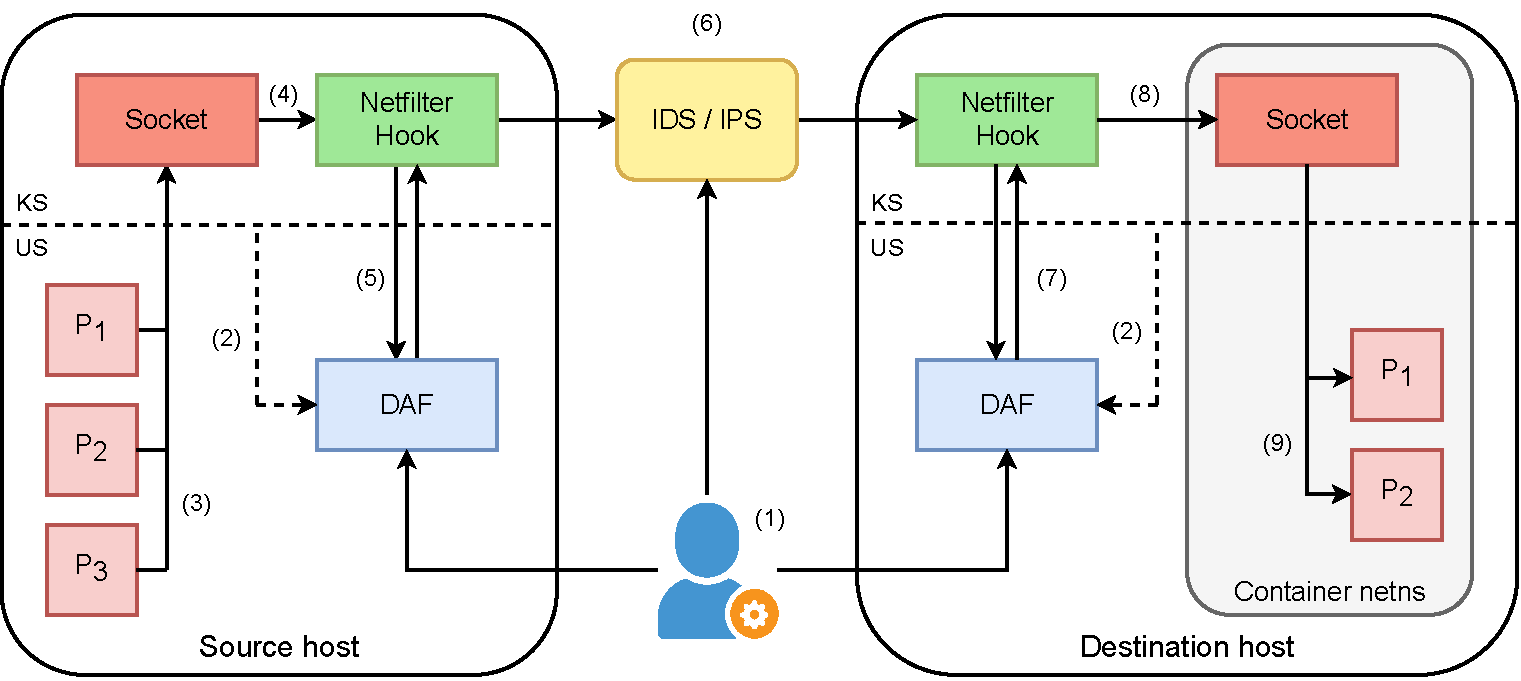
\includegraphics[width=0.8 \textwidth,keepaspectratio]{figures/daf-sys-architecture.pdf}
    \caption{Tagged packet data path. Both endpoints utilize \daf{}.}
    \label{appfw:daf:fig:sys-architecture}
\end{figure}

In order to correlate a process with its specific network traffic, we have identified multiple possibilities:
\begin{itemize}
    \item When considering a threat model where the attacker has limited user-level privileges, \daf{} can be implemented as an extension to the current firewall mechanisms (e.g., \texttt{iptables}), with no intervention on the kernel. This is our main implementation detailed in this paper on Linux.
    \item If we assume an attacker with elevated privileges, \daf{} requires a kernel level implementation, similar with existing antivirus solutions. We have implemented this model on Windows as a proof of concept.
    \item Alternatively, if we regard the attacker as capable of gaining control of his immediate environment but unable to break container isolation, \daf{} can safely run in userspace, in a superior namespace.
    \item If we assume that the attacker has kernel-level privileges and there is no support for virtualization-based solutions, \daf{} can either be implemented on an external hardware token or in a Trusted OS. The former implies that network traffic can no longer be attributed to a certain process due to the lack to OS-level information, but can still be attributed to a certain host and prevent spoofing. Meanwhile, the latter would require hardware support for separating trusted and untrusted protection domains (e.g., ARM TrustZone). These use-cases are outside the scope of this paper.
\end{itemize}

\section{Evaluation}

\subsection{Experimental setup}

The experiments described in this section have been carried out on the following hardware:

\begin{itemize}
    \item \textbf{Intel NUC:} Intel Core i7-7567U CPU @3.50GHz, Intel I219-V 1-Gigabit Ethernet Controller, 8GB DDR4 memory @2400MT/s.
    \item \textbf{IBM System x3550 M4:} Intel Xeon E5-2650Lv2 CPU @1.70GHz, Intel 82599ES 10-Gigabit SFP+ Ethernet Controller, 32GB DDR3 memory @1600MT/s.
\end{itemize}

The reported throughput was derived from the \texttt{iperf3} output and was based on the application data transfer, excluding any headers. Both systems are running a minimal installation of Arch Linux with kernel version 6.7.0. We note that the \textit{rootfs} of the IBM server was network mounted. However, due to file buffering and file system syncs being transmitted on a different 1-Gigabit interface, this fact does not impact our experiments.

\subsubsection{Optimizations and trade-offs}
\label{appfw:daf:optimizations}

During the development of \daf{}, in an effort to achieve a satisfying performance, we were confronted with a number of potential trade-offs. Although some had the capacity to improve throughput by up to an order of magnitude, each would incur a reduction in our security guarantees. Consequently, we decided to implement these optimizations as either build-time or run-time user options. Following is a list of said optimizations, as well as their associated CLI invocation flag.

\begin{itemize}
    \item \textbf{Rescan prevention (R):} During the analysis of each packet, avoid scanning the virtual address space of each potential originator process, except during its initial identification. Subsequent queries will utilize the process state as it was ascertained during its first packet emission or reception. Dynamically loaded objects will not be accounted for.

    \item \textbf{Skip namespace switches (S):} Prevent switching network namespaces on consecutive rule evaluations that reference the same netns symlink. The symlink in question belonging to \textit{procfs} would not be an issue in and of itself. However, external references to said symlink are often used in order to prevent the kernel from deleting the namespace after all processes belonging to it have terminated. This principle can be found implemented in the \texttt{netns} subcommand of \texttt{iproute2}.

    \item \textbf{Disable cached object ordering (build-time; U):} In order to match packets using an aggregate hash that is representative for a certain program, the comprising objects must be arranged in a deterministic manner. To this end, we decided to sort them alphabetically based on their absolute paths. In our implementation, we cache the hashes of all objects belonging to a process as an unordered set, where operations have an average constant-time complexity. When retrieved by the Process Pool Analysis component, an ordered set (logarithmic complexity) is initialized from the contents of the unordered set, relying on its key comparison implementation to order the elements. During our experiments we discovered that we have initially underestimated the cost of this operation. As a result, we offer the choice of working directly with the unordered set in exchange for the ability to match whole programs, not just individual objects.

    \item \textbf{Batch verdict communication (b, B):} During our experiments we concluded that the packet data transfer between kernel space and user space is not a costly operation in and of itself. On the other hand, reporting the verdict for a given packet back to the \texttt{Netfilter Queue} module would block the process for what would at times amount to approx. 30\% of the total execution time. As a result, we decided to implement a verdict batching mechanism. Although capable of significantly improving the performance of \daf{}, we note that this optimization is not as straightforward to utilize as the previously described ones, its performance being contingent on the type of processed traffic. Thus, we define user-adjustable upper limits for both the number of batched packets, and the amount of time that the verdict of any packet is allowed to be delayed (see Subsection \ref{appfw:daf:queuq-verdict-batch-tuning}). Albeit difficult to suggest generic values that would guarantee an adequate performance increase regardless of the type of workload, we found it prudent to carry out forced verdict transmissions whenever a TCP SYN or TCP PSH is encountered. The reason behind the former is to avoid delaying the establishment of new TCP connections. As for the latter, postponing the transfer of what is expected to be a complete message to the endpoint process could provoke unwanted transmission delays at the application level.
\end{itemize}

\subsection{Netfilter Queue tuning}

When selecting the parameters for the \textbf{batched verdict communication optimization (b,B)}, we first determine the lower bounds for the maximum batch size and transmission timeout. Choosing the values for either of these parameters while falling short of this threshold can detract from the performance improvement of the optimization, to the point of completely negating it (e.g. size=1).

\begin{figure}[h]
    % Batch Size (b) impact on Throughput
    \begin{tikzpicture}
        % Throughput
        \begin{axis}[
            axis y line*      = left,
            width             = 0.9\textwidth,
            height            = 4.5cm,
            xmajorgrids       = true,
            ymin              = 4500,
            ymax              = 9500,
            xmin              = 1,
            xmax              = 50,
            xlabel            = {Batch size (b) [pkts]},
            ylabel            = {Throughput [Mbps]},
            % xticklabel style  = {rotate=45},
            xtick distance    = 5,
            ytick             = {5000, 7000, 9000},
            legend columns    = 3,
            legend entries    = {Min-Max throughput,
                                 Average throughput,
                                 Standard deviation},
            legend style      = {at={(-0.03,1.15)}, anchor=south west}
        ]
            % legend images (\addlegendentry fucks with fill plot)
            \addlegendimage{no marks, Green}
            \addlegendimage{no marks, RoyalBlue}
            \addlegendimage{no marks, Red}

            % Minimums and Maximums
            \addplot[name path=lower, color=Green, very thick]
                table[x=pkts, y=min, col sep=comma]
                {src/chapters/04-AppIdFirewall/data/batch-size.csv};
            \addplot[name path=upper, color=Green, very thick]
                table[x=pkts, y=max, col sep=comma]
                {src/chapters/04-AppIdFirewall/data/batch-size.csv};

            % Fill between Minimum and Maximum plots
            \addplot[pattern=north east lines,pattern color=Green] fill between[of=lower and upper];

            % Average
            \addplot[color=RoyalBlue, very thick]
                table[x=pkts, y=avg, col sep=comma]
                {src/chapters/04-AppIdFirewall/data/batch-size.csv};
        \end{axis}

        % Standard Deviation
        \begin{axis}[
            axis y line*      = right,
            x axis line style = {opacity=0},
            xmajorticks       = false,
            width             = 0.9\textwidth,
            height            = 4.5cm,
            xmin              = 1,
            xmax              = 50,
            % ymin              = 0.3,
            % ymax              = 2,
            ylabel            = {Std. Dev. [Mbps]},
        ]
            \addplot[color=Red, very thick]
                table[x=pkts, y=stdev, col sep=comma]
                {src/chapters/04-AppIdFirewall/data/batch-size.csv};
        \end{axis}
    \end{tikzpicture}

    % Batch Timeout (B) impact on Throughput
    \begin{tikzpicture}
        % Throughput
        \begin{axis}[
            axis y line*      = left,
            width             = 0.9\textwidth,
            height            = 4.5cm,
            xmajorgrids       = true,
            ymin              = 4500,
            ymax              = 9500,
            xmin              = 1,
            xmax              = 50,
            xlabel            = {Timeout (B) [$\mu{}s$]},
            ylabel            = {Throughput [Mbps]},
            % xticklabel style  = {rotate=45},
            xtick distance    = 5,
            ytick             = {5000, 7000, 9000},
        ]
            % Minimums and Maximums
            \addplot[name path=lower, color=Green, very thick]
                table[x=time, y=min, col sep=comma]
                {src/chapters/04-AppIdFirewall/data/batch-time.csv};
            \addplot[name path=upper, color=Green, very thick]
                table[x=time, y=max, col sep=comma]
                {src/chapters/04-AppIdFirewall/data/batch-time.csv};

            % Fill between Minimum and Maximum plots
            \addplot[pattern=north east lines,pattern color=Green] fill between[of=lower and upper];

            % Average
            \addplot[color=RoyalBlue, very thick]
                table[x=time, y=avg, col sep=comma]
                {src/chapters/04-AppIdFirewall/data/batch-time.csv};
        \end{axis}

        % Standard Deviation
        \begin{axis}[
            axis y line*      = right,
            x axis line style = {opacity=0},
            xmajorticks       = false,
            width             = 0.9\textwidth,
            height            = 4.5cm,
            xmin              = 1,
            xmax              = 50,
            % ymin              = 0.3,
            % ymax              = 2,
            ylabel            = {Std. Dev. [Mbps]},
        ]
            \addplot[color=Red, very thick]
                table[x=time, y=stdev, col sep=comma]
                {src/chapters/04-AppIdFirewall/data/batch-time.csv};
        \end{axis}
    \end{tikzpicture}

    \caption{Influence of verdict batch size \& timeout on throughput.}
    \label{appfw:daf:fig:batching}
\end{figure}


In order to empirically determine the aforementioned thresholds, we performed six rounds of experiments, varying the maximum batch size by 1 packet and the timeout by 1$\mu{}s$ in the 1-100 range (thus obtaining a dataset of 60,000 throughput values). Figure \ref{appfw:daf:fig:batching} illustrates the impact of each of the two tuning parameters via the average throughput on a 10Gbps link with constant MTU. In order to exemplify the effect of one tuning parameter independently from the other, the dimensions corresponding to the second parameter as well as the experiment round had to be collapsed. Consequently, each average throughput data point was calculated over a subset of 600 values representing the splice obtained from fixing the value on the abscissa.

For the minimum-maximum intervals we decided to fix both the experiment round and one of the tuning parameters, in order to then average the per-experiment minimums and maximums. The motive behind this was to de-emphasize outliers. To compensate for this and correctly represent the throughput variations, we included the standard deviation obtained from the same data slice that was used to calculate the average throughput. Here, we mention that the value range for both plots was truncated to 1-50 in order to better illustrate the impact of suboptimal parameter choices. The subsets used in the calculation of the average throughputs have not been proportionately truncated.

\begin{figure}[h]
    \begin{tikzpicture}
        \begin{axis}[
            width             = \textwidth,
            height            = 7cm,
            at                = {(0,0)},
            xmin              = 5500,
            xmax              = 9710,
            ymax              = 6300,
            xtick distance    = 1000,
            grid              = both,
            xlabel            = {MTU [bytes]},
            ylabel            = {Throughput [Mbps]},
            legend style      = {at={(0.04,0.80)}, anchor=west},
            legend cell align = left,
        ]
            \addplot[color=RoyalBlue, very thick]
                table[x=mtu, y=RUSuPb-doubling, col sep=comma]
                {src/chapters/04-AppIdFirewall/data/cocos-aliasing.csv};
            \addlegendentry{doubling}

            \addplot[color=LimeGreen, very thick]
                table[x=mtu, y=RUSuPb, col sep=comma]
                {src/chapters/04-AppIdFirewall/data/cocos-aliasing.csv};
            \addlegendentry{normal}
        \end{axis}
    \end{tikzpicture}

    \caption{Effect of introducing dynamic resizing of Netlink socket buffer.}
    \label{appfw:daf:fig:aliasing}
\end{figure}


One other value that we concluded needed to be fine tuned is the \textbf{Netlink socket receive buffer size}. While this socket is used for communication between userspace and the \texttt{Netfilter Queue} kernel driver, its receive buffer is also used to store packets that are pending a verdict, only to later be reintroduced in the network stack. In the eventuality that this buffer fills (a common occurrence when the userspace application is slow to reach a verdict) new packets are discarded and the following \texttt{read()} operation fails with the \texttt{ENOBUFS} error code, as an informative measure. Ignoring this problem can lead to aliasing issues that normally manifest as illustrated in Figure \ref{appfw:daf:fig:aliasing}. Insufficient TCP socket buffer sizes may also lead to similar performance downgrades. In response to these events, we assess the current Netlink socket buffer size and double it. This action is performed using the \texttt{SO\_RCVBUFFORCE} socket option as to override the system maximum socket size. We note that after doubling the buffer size from userspace, the kernel doubles it once more in order to allow for bookkeeping overhead.

\subsubsection{Performance analysis}

Our performance analysis of \daf{} is primarily based on \texttt{iperf3} throughput tests between a client running our firewall and a server on another identical host. The two hosts are directly linked, with no additional equipment serving as middleboxes. We note that the values we report represent the average throughput over 10s sessions, averaged once more over 10 and 5 rounds of experiments on the IBM server and NUC system respectively. On the 10-Gigabit servers, we decided to manually increase the default and maximum TCP socket buffer sizes, a common practice in such cases. Although in our final reports these are set to 32MB, we did not perceive any noticeable performance gain for values higher than 8MB. The NUC desktop computers utilize the default maximums of 4MB for the send buffer and 6MB for the receive buffer.

\begin{figure}[h]
    \centering

    \begin{tikzpicture}
        \begin{axis}[
            width             = \textwidth,
            height            = 6cm,
            at                = {(0,0)},
            xmin              = 600,
            xmax              = 9300,
            ymin              = 0,
            xtick distance    = 2000,
            grid              = both,
            xlabel            = {MTU [bytes]},
            ylabel            = {Throughput [Mbps]},
            legend style      = {at={(0.97,0.15)}, anchor=east},
            legend cell align = left,
        ]
            \addplot[color=RoyalBlue, very thick]
                table[x=mtu, y=sigRUS-usenix, col sep=comma]
                {src/chapters/05-SignatureFirewall/data/cocos-throughput.csv};
            \addlegendentry{RUS+sig (epoll)}

            \addplot[color=OliveGreen, very thick]
                table[x=mtu, y=sigRUS-esorics, col sep=comma]
                {src/chapters/05-SignatureFirewall/data/cocos-throughput.csv};
            \addlegendentry{RUS+sig (io\_uring)}
        \end{axis}
    \end{tikzpicture}

    \caption{\daf{} throughput on the IBM system with signature-based packet tagging.}
    \label{sign:linux:fig:cocos-throughput}
\end{figure}


Figure \ref{appfw:daf:fig:cocos-throughput} illustrates the performance gain of each optimization. Here, we note the exceedingly high variations. We attribute these to the use of the \texttt{io\_uring} interface for asynchronous I/O operations. In our implementation, we decided to launch a kernel thread on a different CPU core that continuously polls the system call submission queue in \daf{}. Prior to this revision, we employed an \texttt{epoll} hierarchization system to permit us the prioritization of certain events (e.g., system state model updates) over other. However, profiling sessions revealed that our firewall spent over 50\% of the time waiting for \texttt{epoll} events, limiting the average throughput with full optimizations to approx. 5.4Gbps. Our experimental results using this version can be found in Figure \ref{appfw:daf:fig:cocos-throughput-epoll}. In it there is an additional optimization, namely \textit{Uniform Prioritization (u)}. This optimization would circumvent the \texttt{epoll} hierarchy in order to give equal chances to both packets and system events to be processed, at the cost of potentially using an outdated system state when reaching a singular packet verdict. Once we transitioned to the \texttt{io\_uring} implementation, this optimization became redundant and was elliminated. As a reulst, bynot only offloading the majority of I/O operations (consisting mostly of packet reads from the netlink socket) to a secondary core but also drastically limiting the amount of context switches between protection domains, we have increased the average throughput to approx. 8.8Gbps. We believe that the gap between this and the baseline throughput can be bridged by extending \texttt{libnetfilter\_queue} to allow asynchronous batched verdict transmission.

\begin{figure}[h]
    \centering

    \begin{tikzpicture}
        \begin{axis}[
            width             = \textwidth,
            height            = 6cm,
            at                = {(0,0)},
            xmin              = 0,
            xmax              = 9710,
            ymin              = 0,
            ymax              = 6,
            xtick distance    = 1000,
            ytick distance    = 1,
            grid              = both,
            xlabel            = {MTU [bytes]},
            ylabel            = {Throughput [Gbps]},
            legend columns    = 7,
            legend style      = {at={(0.05,1.05)}, anchor=south west}
        ]
            \addplot[color=Goldenrod, very thick]
                table[x=mtu, y=baseline, col sep=comma]
                {src/chapters/04-AppIdFirewall/data/cocos-throughput.csv};
            \addlegendentry{baseline}

            \addplot[color=Rhodamine, very thick]
                table[x=mtu, y=vanilla, col sep=comma]
                {src/chapters/04-AppIdFirewall/data/cocos-throughput-epoll.csv};
            \addlegendentry{unopt}

            \addplot[color=Red, very thick]
                table[x=mtu, y=R, col sep=comma]
                {src/chapters/04-AppIdFirewall/data/cocos-throughput-epoll.csv};
            \addlegendentry{R}

            \addplot[color=Purple, very thick]
                table[x=mtu, y=RU, col sep=comma]
                {src/chapters/04-AppIdFirewall/data/cocos-throughput-epoll.csv};
            \addlegendentry{RU}

            \addplot[color=Green, very thick]
                table[x=mtu, y=RUS, col sep=comma]
                {src/chapters/04-AppIdFirewall/data/cocos-throughput-epoll.csv};
            \addlegendentry{RUS}

            \addplot[color=RoyalBlue, very thick]
                table[x=mtu, y=RUSu, col sep=comma]
                {src/chapters/04-AppIdFirewall/data/cocos-throughput-epoll.csv};
            \addlegendentry{RUSu}

            \addplot[color=Orange, very thick]
                table[x=mtu, y=RUSuPb, col sep=comma]
                {src/chapters/04-AppIdFirewall/data/cocos-throughput-epoll.csv};
            \addlegendentry{RUSuB}
        \end{axis}
    \end{tikzpicture}

    \caption{\daf{} throughput on IBM system (\texttt{epoll} version).}
    \label{appfw:daf:fig:cocos-throughput-epoll}
\end{figure}


In the same figure we also depict the throughput of \daf{} on the 10-Gigabit server while also calculating and attaching SHA256-HMACs of the Layer 4 payload as IP options. Notice how we forgo the use of verdict batching since it would not permit us to re-inject the modified packet into the kernel, strictly due to a \texttt{Netfilter Queue} API limitation. Once again, we believe that this limitation could be alleviated by adding a simultaneous packet override through an \texttt{iov} interface. However, this would also require changes not only to \texttt{libnetfilter\_queue} but also the \texttt{Netfilter Queue} driver, both of which we conside outside the scope of this paper. During this experiment we manually enforced a smaller Maximum Segment Size (MSS) for \texttt{iperf3} in order to ensure that the newly introduced 36-byte IP options section would not exceed the MTU at any given time. Note however, that \texttt{iperf3} clamps the MSS values within the 88-9216 range, thus leading to severe performance downgrades due to fragmentation. Under these conditions, we register a peak average throughput of approx. 835Mbps.

